% !TEX root = task-2-4-3.tex
% Editable task bank. Append new BankTask blocks at the end of the document.
\documentclass[12pt,a4paper]{article}
\usepackage{physics-textbook}
\usepackage{graphicx,needspace}
\usetikzlibrary{decorations.pathmorphing}
\newif\ifShowSolutions
\ifdefined\TutorEdition
  \ShowSolutionstrue
\else
  \ShowSolutionsfalse % Change to \ShowSolutionstrue to display solutions.
\fi
\newcounter{banktask}
\newsavebox{\BankTaskBox}
\newcommand{\BankTaskContent}[3]{%
  \noindent\textbf{\thebanktask.}\quad #2\par
  \ifShowSolutions
    \Needspace{50mm}% Keep the solution heading with its opening text or diagram.
    #3\par
    \ifdefined\TutorEdition
      \ifcsname TutorSource#1\endcsname
        \nopagebreak\smallskip{\small\csname TutorSource#1\endcsname\par}%
      \fi
    \fi
  \fi
}
\newcommand{\BankTask}[3]{%
  \refstepcounter{banktask}\par\medskip
  \sbox{\BankTaskBox}{\begin{minipage}{\linewidth}%
    \BankTaskContent{#1}{#2}{#3}\end{minipage}}%
  \ifdim\dimexpr\ht\BankTaskBox+\dp\BankTaskBox\relax>\dimexpr\textheight-20mm\relax
    \Needspace{35mm}\BankTaskContent{#1}{#2}{#3}%
  \else
    \Needspace{\dimexpr\ht\BankTaskBox+\dp\BankTaskBox\relax}%
    \noindent\usebox{\BankTaskBox}\par
  \fi
  \medskip
}
\begin{document}
\BookSubsection{2.4.3}{Температурная шкала. Абсолютная температура}


% Source sdamgia-801: https://phys-ege.sdamgia.ru/problem?id=801
\BankTask{sdamgia-801}{
Значение температуры по шкале Цельсия, соответствующее абсолютной температуре $10$ $K$, равно:

$1$) $- 273 ^\circ$ 

$2$) $- 263 ^\circ$ 

$3$) $263 ^\circ$ 

$4$) $283 ^\circ$
}{
\smallskip\noindent\textbf{Решение}\par
Нулю градусов по шкале Кельвина соответствует $- 273 ^{\circ} C,$ а по величине $1K=1 ^{\circ} C.$ Таким образом, температуре в $10$ $K$ соответствует $- 273 ^{\circ} C + 10 ^{\circ} C= - 263 ^{\circ} C.$

Ответ: $2$.
}

% Source sdamgia-808: https://phys-ege.sdamgia.ru/problem?id=808
\BankTask{sdamgia-808}{
Какова температура кипения воды при нормальном атмосферном давлении по абсолютной шкале температур?

$1$) $100$ $K$

$2$) $173$ $K$

$3$) $273$ $K$

$4$) $373$ $K$
}{
\smallskip\noindent\textbf{Решение}\par
Нулю градусов в шкале Цельсия ($0^\circ$C) соответствует абсолютная температура $273$ $K$, а по величине $1\,\text{К}=1^\circ$С. Таким образом, температуре в $100^\circ$C соответствует абсолютная температура $273$ + $100=373\,\text{К}$.

Ответ: $4$.
}

% Source sdamgia-3204: https://phys-ege.sdamgia.ru/problem?id=3204
\BankTask{sdamgia-3204}{
Температура кипения азота по абсолютной шкале температур Кельвина составляет $77\,\text{К}$. Чему равна эта температура по шкале Цельсия?

$1$) $77 ^\circ\text{C};$

$2$) ) $- 77 ^\circ\text{C};$

$3$) $- 196 ^\circ\text{C};$

$4$) $350 ^\circ\text{C}.$
}{
\smallskip\noindent\textbf{Решение}\par
Нулю градусов по шкале Кельвина соответствует $- 273 ^\circ\text{C},$ а по величине $1K=1 ^\circ\text{C}.$ Таким образом, температуре в $77K$ соответствует $- 273 ^\circ\text{C} + 77 ^\circ\text{C}= - 196 ^\circ\text{C}.$

Ответ: $3$.
}

% Source sdamgia-3210: https://phys-ege.sdamgia.ru/problem?id=3210
\BankTask{sdamgia-3210}{
Согласно расчетам, температура жидкости должна быть равна $187\,\text{К}$. Между тем термометр в сосуде показывает температуру $- 86 ^\circ\text{C}.$ Это означает, что 

$1$) термометр показывает более низкую температуру

$2$) термометр показывает более высокую температуру

$3$) термометр показывает расчетную температуру

$4$) термометр не рассчитан на низкие температуры и требует замены
}{
\smallskip\noindent\textbf{Решение}\par
Для того, чтобы сравнивать физические величины, их необходимо выразить в одинаковых единицах измерения. Определим, каковы показания термометра по абсолютной шкале температур. Нулю градусов по шкале Цельсия соответствует $273K,$ а по величине $1K=1 ^\circ\text{C}.$ Следовательно, температуре $( - 86 ^\circ\text{C} )$ соответствует $273K - 86K=187K.$ Таким образом, термометр показывает расчетную температуру.

Ответ: $3$.
}

% Source sdamgia-3322: https://phys-ege.sdamgia.ru/problem?id=3322
\BankTask{sdamgia-3322}{
\begin{center}\begin{tikzpicture}[task graph]
\draw[task curve,rounded corners=8pt] (0,-1.1) rectangle (7.5,1.1);\draw[task curve] (0,-.15)--(7.5,-.15) (0,-.4)--(7.5,-.4);\fill (2.6,-.4) rectangle (7.5,-.15);\foreach \x in {.2,.6,...,7.4}{\draw[task tick] (\x,-.15)--(\x,.55);}\foreach \x/\s in {1/30,3/20,5/10,7/0}{\draw[task curve] (\x,-.15)--(\x,.95);\node[below] at (\x,-.45) {$\s$};}
\end{tikzpicture}\end{center}
На рисунке показана часть шкалы комнатного термометра (проградуированного в градусах Цельсия). Определите абсолютную температуру воздуха в комнате.

$1$) $21^\circ$C

$2$) $23^\circ$C

$3$) $275\,\text{К}$

$4$) $295\,\text{К}$
}{
\smallskip\noindent\textbf{Решение}\par
В комнатном термометре используется шкала температур Цельсия. Определим цену деления шкалы градусника: $\frac{30 ^{\circ} C - 20 ^{\circ} C}{5} =2 ^{\circ} C.$ Следовательно, по шкале Цельсия температура в комнате равна $t=22 ^{\circ} C.$ Нулю градусов по шкале Цельсия соответствует температура $273K,$ а по величине $1K=1 ^{\circ} C.$ Таким образом, температуре в $t=22 ^{\circ} C$ соответствует абсолютная температура $273K + 22K=295K.$

Ответ: $4$.
}

% Source sdamgia-5719: https://phys-ege.sdamgia.ru/problem?id=5719
\BankTask{sdamgia-5719}{
В таблице приведены характеристики четырех жидкостей

\begin{center}\begin{tabular}{|p{0.287\linewidth}|p{0.287\linewidth}|p{0.287\linewidth}|}\hline
Жидкость & Плотность, $\text{кг}/\text{м}^{3}$ & Температура \newline замерзания, $K$\\\hline
Вода & $1000$ & $273$\\\hline
Спирт & $800$ & $159$\\\hline
Ртуть & $13600$ & $234$\\\hline
Антифриз & $1050$ & $253$\\\hline\end{tabular}\end{center}

Самая низкая температура на поверхности земли (-$89{,}2^\circ$C) была зарегистрирована в $1983$ года на советской научной станции Восток в Антарктиде. Для измерения такой температуры можно было использовать термометр, наполненный

$1$) водой

$2$) спиртом

$3$) ртутью

$4$) антифризом
}{
\smallskip\noindent\textbf{Решение}\par
Абсолютная температура связана с температурой по шкале Цельсия соотношением$T = t$ + $273$, значит, самая низкая температура в кельвинах равна $183{,}8$ $K$. Эта температура могла быть зафиксирована, если температура замерзания жидкости в термометре ниже значения данной температуры. По таблице находим, что этому требованию удовлетворяет спирт.

Правильный ответ указан под номером $2$.
}

% Source sdamgia-9735: https://phys-ege.sdamgia.ru/problem?id=9735
\BankTask{sdamgia-9735}{
При построении температурной шкалы Реомюра принимается, что при нормальном атмосферном давлении лед тает при температуре $0$ градусов Реомюра (°$R$), а вода кипит при температуре $80^\circ$R. Найдите, чему равна средняя кинетическая энергия поступательного теплового движения частицы идеального газа при температуре $91^\circ$R. (В электрон-вольтах; округлите до сотых долей.)
}{
\smallskip\noindent\textbf{Решение}\par
Из описания следует, что один градус шкалы Реомюра соответствует $\frac{100}{80} =1{,}25 ^\circ\text{C} .$

Соответственно, $91 ^\circ R$ — это $100 + 11 \cdot 1{,}25 = 113{,}75 ^\circ\text{C}$ или $113{,}75 + 273=386{,}75\text{К}.$

Средняя кинетическая энергия теплового движения частиц идеального газа связана с температурой соотношением: 

$\overline{E}_{\text{к}} = \frac{3}{2} kT=1{,}5 \cdot 1{,}38 \cdot 10 ^{- 23} \text{Дж}/\text{К} \cdot 386{,}75\text{К}\approx8 \cdot 10 ^{- 21} \text{Дж}\approx 0{,}05\text{эВ}.$ 

Ответ: $0{,}05$.
}

% Source sdamgia-9757: https://phys-ege.sdamgia.ru/problem?id=9757
\BankTask{sdamgia-9757}{
Для получения и поддержания температуры $0^\circ$С, одной из двух реперных точек на шкале Цельсия, в лабораторной практике часто используют следующий метод. В теплоизолированный стакан наливают дистиллированную воду комнатной температуры, поливают воду сверху жидким азотом, перемешивая смесь ложкой до тех пор, пока не образуется масса серого цвета, состоящая из мелких кристалликов льда и воды. Это обеспечивает нужную температуру в течение длительного времени — смесь помещают в сосуд Дьюара, где она медленно тает при $0^\circ$С. Какой объем $V$ жидкого азота требуется израсходовать для получения массы $m=300\,\text{г}$ такой смеси, содержащей $75$\% льда и $25$\% воды (по массе), из воды при $25^\circ$С? Теплоемкостями стакана и ложки, а также потерями теплоты можно пренебречь. Плотность жидкого азота $\rho _{\text{ж}}=808\,\text{кг}$/$\text{м}^{3}$, удельная теплота парообразования $L=197{,}6\,\text{кДж}$/кг.
}{
\smallskip\noindent\textbf{Решение}\par
$1$. Из условия задачи понятно, что происходит в системе при получении смеси льда и воды, реализующей реперную точку шкалы Цельсия — $0^\circ$С. Сначала вся масса воды с удельной теплоемкостью $c_{\text{в}}$ охлаждается от $25^\circ$С до $0^\circ$С на $\Delta T=25^\circ$С, а затем $75$\% массы воды превращается в лед при температуре $0^\circ$С, отдавая свою теплоту кристаллизации (удельная теплота кристаллизации воды $\lambda$ равна удельной теплоте плавления льда). В этом процессе отданное водой количество теплоты равно:

$Q = c_{\text{в}} \cdot m \cdot \Delta T + \lambda \cdot ( 3m/4 ) = 4200 \cdot 0{,}3 \cdot 25 + 3{,}3 \cdot 10 ^{5} \cdot 0{,}225 = 105{,}75\,\text{кДж}$.

$2$. Теплота $Q$, отбираемая от воды в данном процессе, идет по условию только на испарение массы $m_{\text{ж}}=\rho _{\text{ж}}\cdot V$ жидкого азота: $Q=mL=\rho_{\text{ж}}VL=808 \cdot 197600V=159660{,}8V\text{кДж}.$

$3$. Таким образом, надо израсходовать объем жидкого азота, равный 

$V=105{,}75$/$159660{,}8$ $\approx$ $6{,}623\cdot 10^{-4}$ $\text{м}^{3}$ $\approx$ $662\,\text{см}^{3}$.

Ответ: $V$ $\approx$ $662\,\text{см}^{3}$.
}


% Source 4C6FA1: https://ege.fipi.ru/bank/questions.php?search=1&proj=BA1F39653304A5B041B656915DC36B38&qid=4C6FA1
\BankTask{4C6FA1}{
Температура неона увеличилась с $27\,{}^{\circ}\text{C}$ до $177\,{}^{\circ}\text{C}$. Во сколько раз увеличилась средняя кинетическая энергия его молекул?
}{
\smallskip\noindent\textbf{Решение от GPT}\par
Абсолютные температуры: $T_1=(27+273)\,\text{К}=300\,\text{К}$, $T_2=(177+273)\,\text{К}=450\,\text{К}$. Поскольку $E=\frac{3}{2}kT$, получаем $\frac{E_2}{E_1}=\frac{450}{300}=1{,}5$. Ответ: в $1{,}5$ раза.
}

% Source E1896D: https://ege.fipi.ru/bank/questions.php?search=1&proj=BA1F39653304A5B041B656915DC36B38&qid=E1896D
\BankTask{E1896D}{
На фотографии изображён спиртовой термометр со шкалой Цельсия. Погрешность измерения температуры при помощи этого термометра равна половине цены деления. Определите абсолютную температуру спирта (в $\text{К}$) в колбе термометра.

\par\begin{center}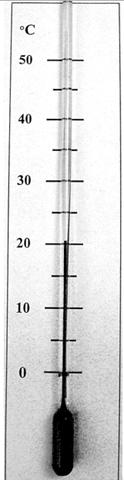
\includegraphics[width=.9\linewidth,height=.48\textheight,keepaspectratio]{_run/photos/5630ecceb8effddffd3091ab131a37434dec32efb2c00debbd378a33ec95d444.png}\end{center}\par
}{
\smallskip\noindent\textbf{Решение от GPT}\par
Термометр показывает $t=20\,^{\circ}\text{C}$, цена деления его шкалы составляет $5\,^{\circ}\text{C}$. Абсолютная температура $T=273+20=293\,\text{К}$, а погрешность $\Delta T=5/2=2{,}5\,\text{К}$. Ответ: $T=(293{,}0\pm2{,}5)\,\text{К}$.
}

\end{document}
